\section{Lessons learned}
%\addcontentsline{toc}{section}{Lessons learned}

\subsection{Monitoring - Performance improvements}
By analyzing metrics, specifically "average request duration by endpoint", and incorporating research conducted by one of the team members, we successfully reduced latency across our endpoints. This improvement is evident in the screenshot below: 
\begin{figure}[H]
    \centering
    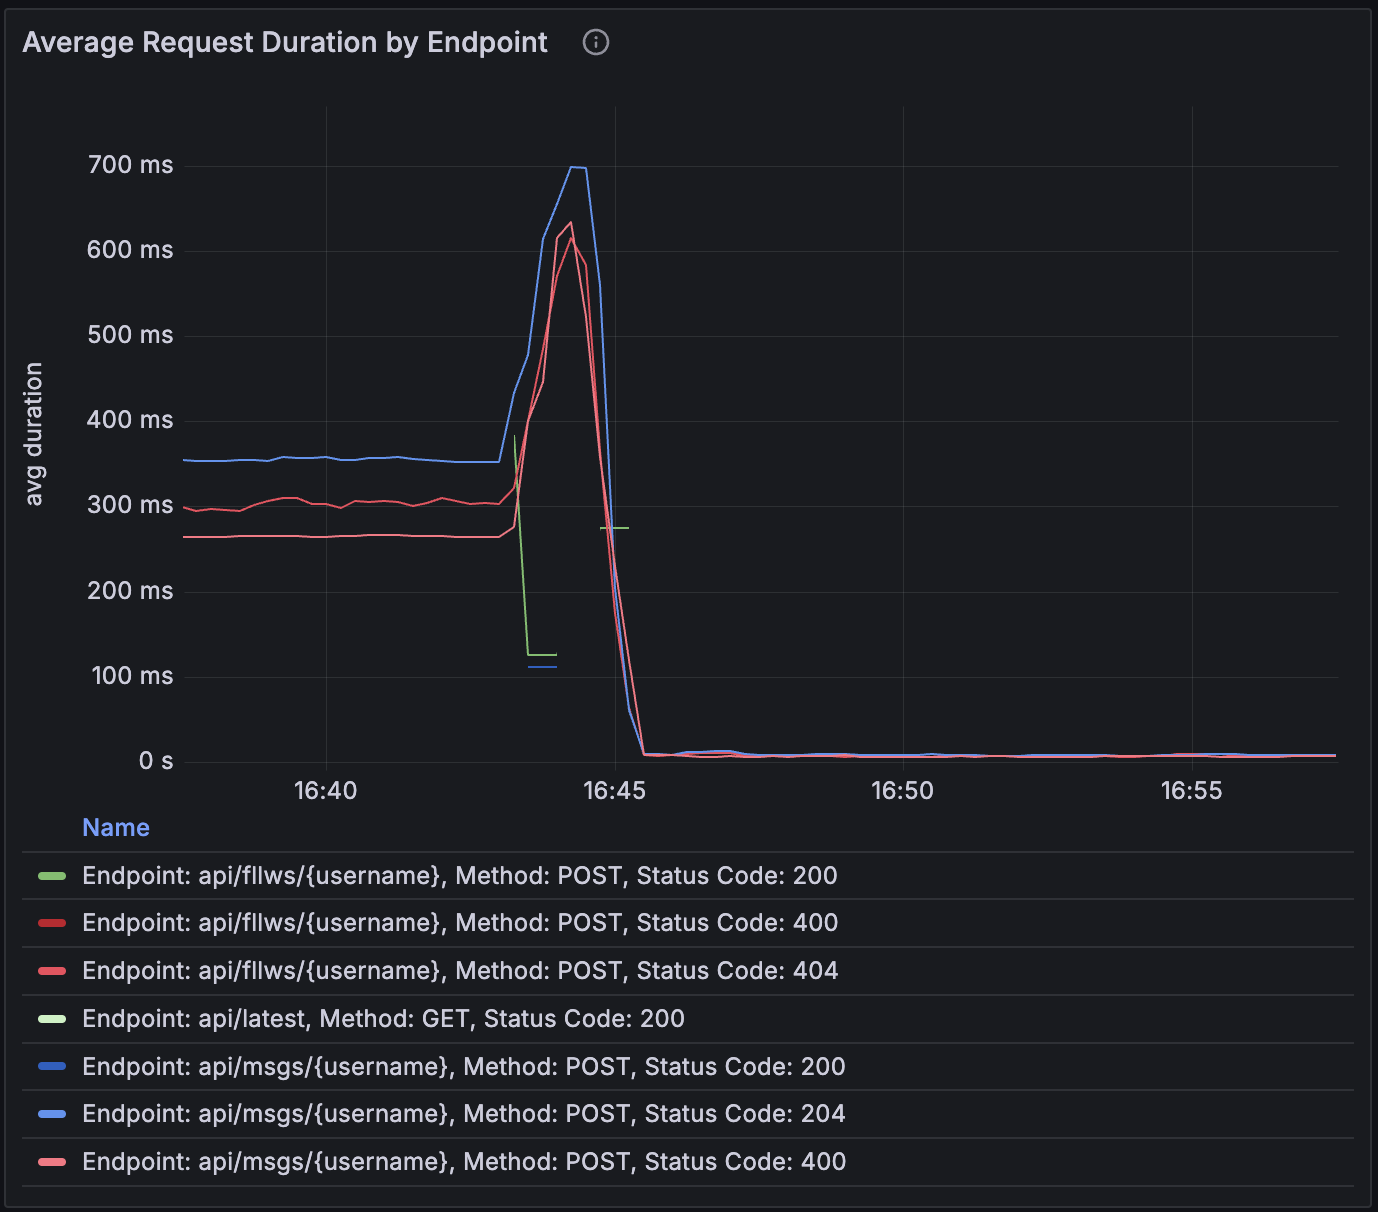
\includegraphics[height=0.9\textwidth]{images/grafana-endpoints-latency.png}
    \caption{Significant reduction of latency metrics measured in Grafana}
    \label{fig:grafana-endpoints-latency}
\end{figure}

The primary cause of the high latency was the geographical separation between our Database (hosted in the NYC region) and our application server (in the FRA region).

Issue link: 

\subsection{Monitoring - Bug fixing}

The follow/unfollow endpoint was returning a 200(OK) status code, instead of 204(NO CONTENT) as requested by the simulator API, resulting in cumulative errors. It was possible to detect that given the information provided by the \href{http://206.81.24.116/status.html}{\color{blue}http://206.81.24.116/status.html} dashboard. 
\\
Issue: Grafana and Loki memory issues
In addressing the disk space overloading issues on our Grafana server where we hosted Loki as well, we utilized DigitalOcean's recovery console to identify and resolve the root cause. By executing the command $sudo lsof +L1$, we detected files that had been deleted but were still held open by processes, which in turn occupied disk space. We terminated these processes using $sudo kill -HUP [PID]$, which released the disk space and restored server functionality, allowing us to regain access to the Grafana platform and establish SSH connecitons to the server. This intervention resolved the memory issue and retored normal operations.

Issue link:


Slow response on the /public endpoint ... ??

Issue link: \href{https://github.com/DevopsGroupC/Minitwit/issues/141}{\color{blue}Look into adding indeces to our database #141}


% Describe the biggest issues, how you solved them, and which are major lessons learned with regards to:

% evolution and refactoring
% operation, and
% maintenance
% of your ITU-MiniTwit systems. Link back to respective commit messages, issues, tickets, etc. to illustrate these.

% Also reflect and describe what was the "DevOps" style of your work. For example, what did you do differently to previous development projects and how did it work?

% The biggest issues: 